\documentclass{article}
\usepackage{graphicx} % Required for inserting images
\usepackage{amsmath}
\setlength{\jot}{10pt} % extra leading between lines of multi-line displays

% Spacing between displayed equations and surrounding text. Appended to \normalsize
% because the display skips are reset on every font size change.
\makeatletter
\g@addto@macro\normalsize{%
    \setlength{\abovedisplayskip}{12pt plus 3pt minus 4pt}%
    \setlength{\belowdisplayskip}{12pt plus 3pt minus 4pt}%
    \setlength{\abovedisplayshortskip}{2pt plus 3pt}%
    \setlength{\belowdisplayshortskip}{8pt plus 3pt minus 4pt}%
}
\makeatother
\usepackage{amsthm}
\usepackage{amssymb}
\usepackage{xcolor}
\usepackage[authoryear]{natbib}
\bibliographystyle{apalike}
\usepackage[font=small,labelfont=bf]{caption}
\usepackage{authblk}
\usepackage[hidelinks]{hyperref}
\usepackage{nameref}
\usepackage[most]{tcolorbox}


\graphicspath{{./figures/}}


\title{Estimating Relative Changes in RNA Polymerase II Elongation, Splicing, and RNA Degradation Kinetics from Total RNA-seq}

\author[1,2]{Jakub Koubele\thanks{Correspondence: \texttt{jkoubele@uni-koeln.de}}}
\author[1,2]{Andreas Beyer\thanks{Correspondence: \texttt{andreas.beyer@uni-koeln.de}}}

\affil[1]{University of Cologne, Faculty of Medicine and University Hospital Cologne, Germany}
\affil[2]{Cologne Excellence Cluster on Cellular Stress Responses in Aging-Associated Diseases (CECAD), University of Cologne, Germany}


\date{}

\begin{document}


    \maketitle

    \begin{abstract}
        Description of what I did.
    \end{abstract}


    \section{Introduction}
    \begin{itemize}
        \item RNA metabolism is dynamic system, speed of reactions = kinetic rates. Kinetic rates are important \citep{furlanDynamicsTranscriptionalPosttranscriptional2021}.
        \begin{itemize}
            \item For example, \citet{vockRNADecayCafeUniformlyProcessed2025} recently estimated that variability in RNA degradation rate explains at least 25\% of variability in transcript abundances between different human cell lines. In immune system, control of RNA decay plays an especially important regulatory role \citep{schottNetworksControllingMRNA2010}.
            \item Transcription elongations speed also plays an important role in RNA metabolism. Changes in Pol II speed can affect several co-transcriptional processes, such as splicing, $\text{m}^{6}$A RNA methylation, and polyadenylation \citep{munizRNAPolymeraseII2021}. Recently, a study of \citet{debesAgeingassociatedChangesTranscriptional2023} showed that organism aging is associated with an increase in Pol II speed, whereas lifespan-prolonging interventions tend to decrease it.
            \item The speed of intron splicing (time needed to splice the intron out of the transcript) is another important aspect of RNA metabolism. The estimates of intron splicing speed varies a lot, ranging from several seconds up to 15 minutes \citep{alpertPerfectTimingSplicing2017, shenasaPremRNASplicingIts2023, sethiSinglemoleculeMultimodalTiming2025}.
            \item I should also discuss transcription initiation rate, it's the main regulator of transcript abundance.
        \end{itemize}
        \item Many other kinetic rates are important, e.g \citet{mullerNuclearExportLimiting2024} recently showed that speed of nuclear export is largely variable and influence the mRNA lifetime. Also translation efficency is widely studied \citep{gingoldDeterminantsTranslationEfficiency2011}, as it affect the proteins abundance. However, our work here will focus only on rates of transcription initiation, elongation, splicing and RNA degradation, as these rates affect total RNA-seq data and we will be able to capture them in our model.
        \item Measuring RNA kinetic rates is challenging, dedicated experiments are needed. Usually, these methods rely on RNA labeling \citep{furlanDynamicsTranscriptionalPosttranscriptional2021}.
        \begin{itemize}
            \item Maybe I can elaborate bit more on these method, but only briefly, as they are not the focus of my work.
        \end{itemize}

        \item Here, we discuss how total RNA-seq can be used to say something about these rates. Total RNA-seq data are common, easy to produce, and large amount of them is already available. However, due to 'static' nature of total RNA-seq data, our measurements will be bit more limited.

    \end{itemize}

    \subsection{Related Work}
    Here we briefly review methods most relevant to our approach; for a more comprehensive overview of computational methods for inferring RNA kinetic rates from sequencing data, we refer the reader to \citet{furlanDynamicsTranscriptionalPosttranscriptional2021}.
    \begin{itemize}
        \item \citet{ameurTotalRNASequencing2011} described the relation between intron coverage and transcription elongation speed in total RNA-seq. This principle was then used in subsequent works which attempted to model transcription elongation speed from total RNA-seq \citep{jonkersGenomewideDynamicsPol2014, kawamuraStatisticalInferenceRate2019, debesAgeingassociatedChangesTranscriptional2023}.
        \item The SnapSHot-Seq method \citep{graySnapShotSeqMethodExtracting2014} also uses shape of intronic coverage, but assumes constant elongation speed, and used the intronic coverage to compute other kinetic rates. Describes intron coverage as mixture of unspliced and nascent introns exactly as I do.
        \item The INSPEcT- method \citep{furlanGenomewideDynamicsRNA2020} is conceptually bit similar to my work, but focuses on between-gene comparison rather than between-conditions comparison.
        \item The EISA method \citep{gaidatzisAnalysisIntronicExonic2015} is more similar to my approach, count intron and exons counts per gene and compute LFC of them between conditions.
        \item The REMBRANDTS method \citep{alkallasInferenceRNADecay2017} builds on EISA, works with assumption that splicing machinery may saturate for highly expressed gene, somehow pools information across genes to remove this bias from EISA-based method.
    \end{itemize}


    \section{Dynamical Model of RNA Metabolism}

    We will now describe a simple dynamical model of RNA metabolism. For a more thorough description of the model and its assumptions, please see the section \nameref{supplementary_methods}. 
    
    Mathematically, the model couples a transport partial differential equation (PDE) for the spatial density of elongating polymerases along the gene with a small set of ordinary differential equations (ODEs) 
    for the abundances of completed (mature) transcripts and unspliced introns.
    

    \subsection{Model Schema and Kinetic Rates}

    The transcription is started by the RNA polymerase binding to the transcription start site (TSS) on DNA. Then, the RNA polymerase transcribes DNA by moving on it, elongating the nascent transcript. Once an intron is fully transcribed, the splicing machinery removes the intron from the transcript and degrades it. Finally, mature transcripts live in the cell, until they are eventually degraded. The schema of this model is visualized in figure \ref{fig:rna_metabolism_schema}.


    \begin{figure}[htbp]
        \centering
        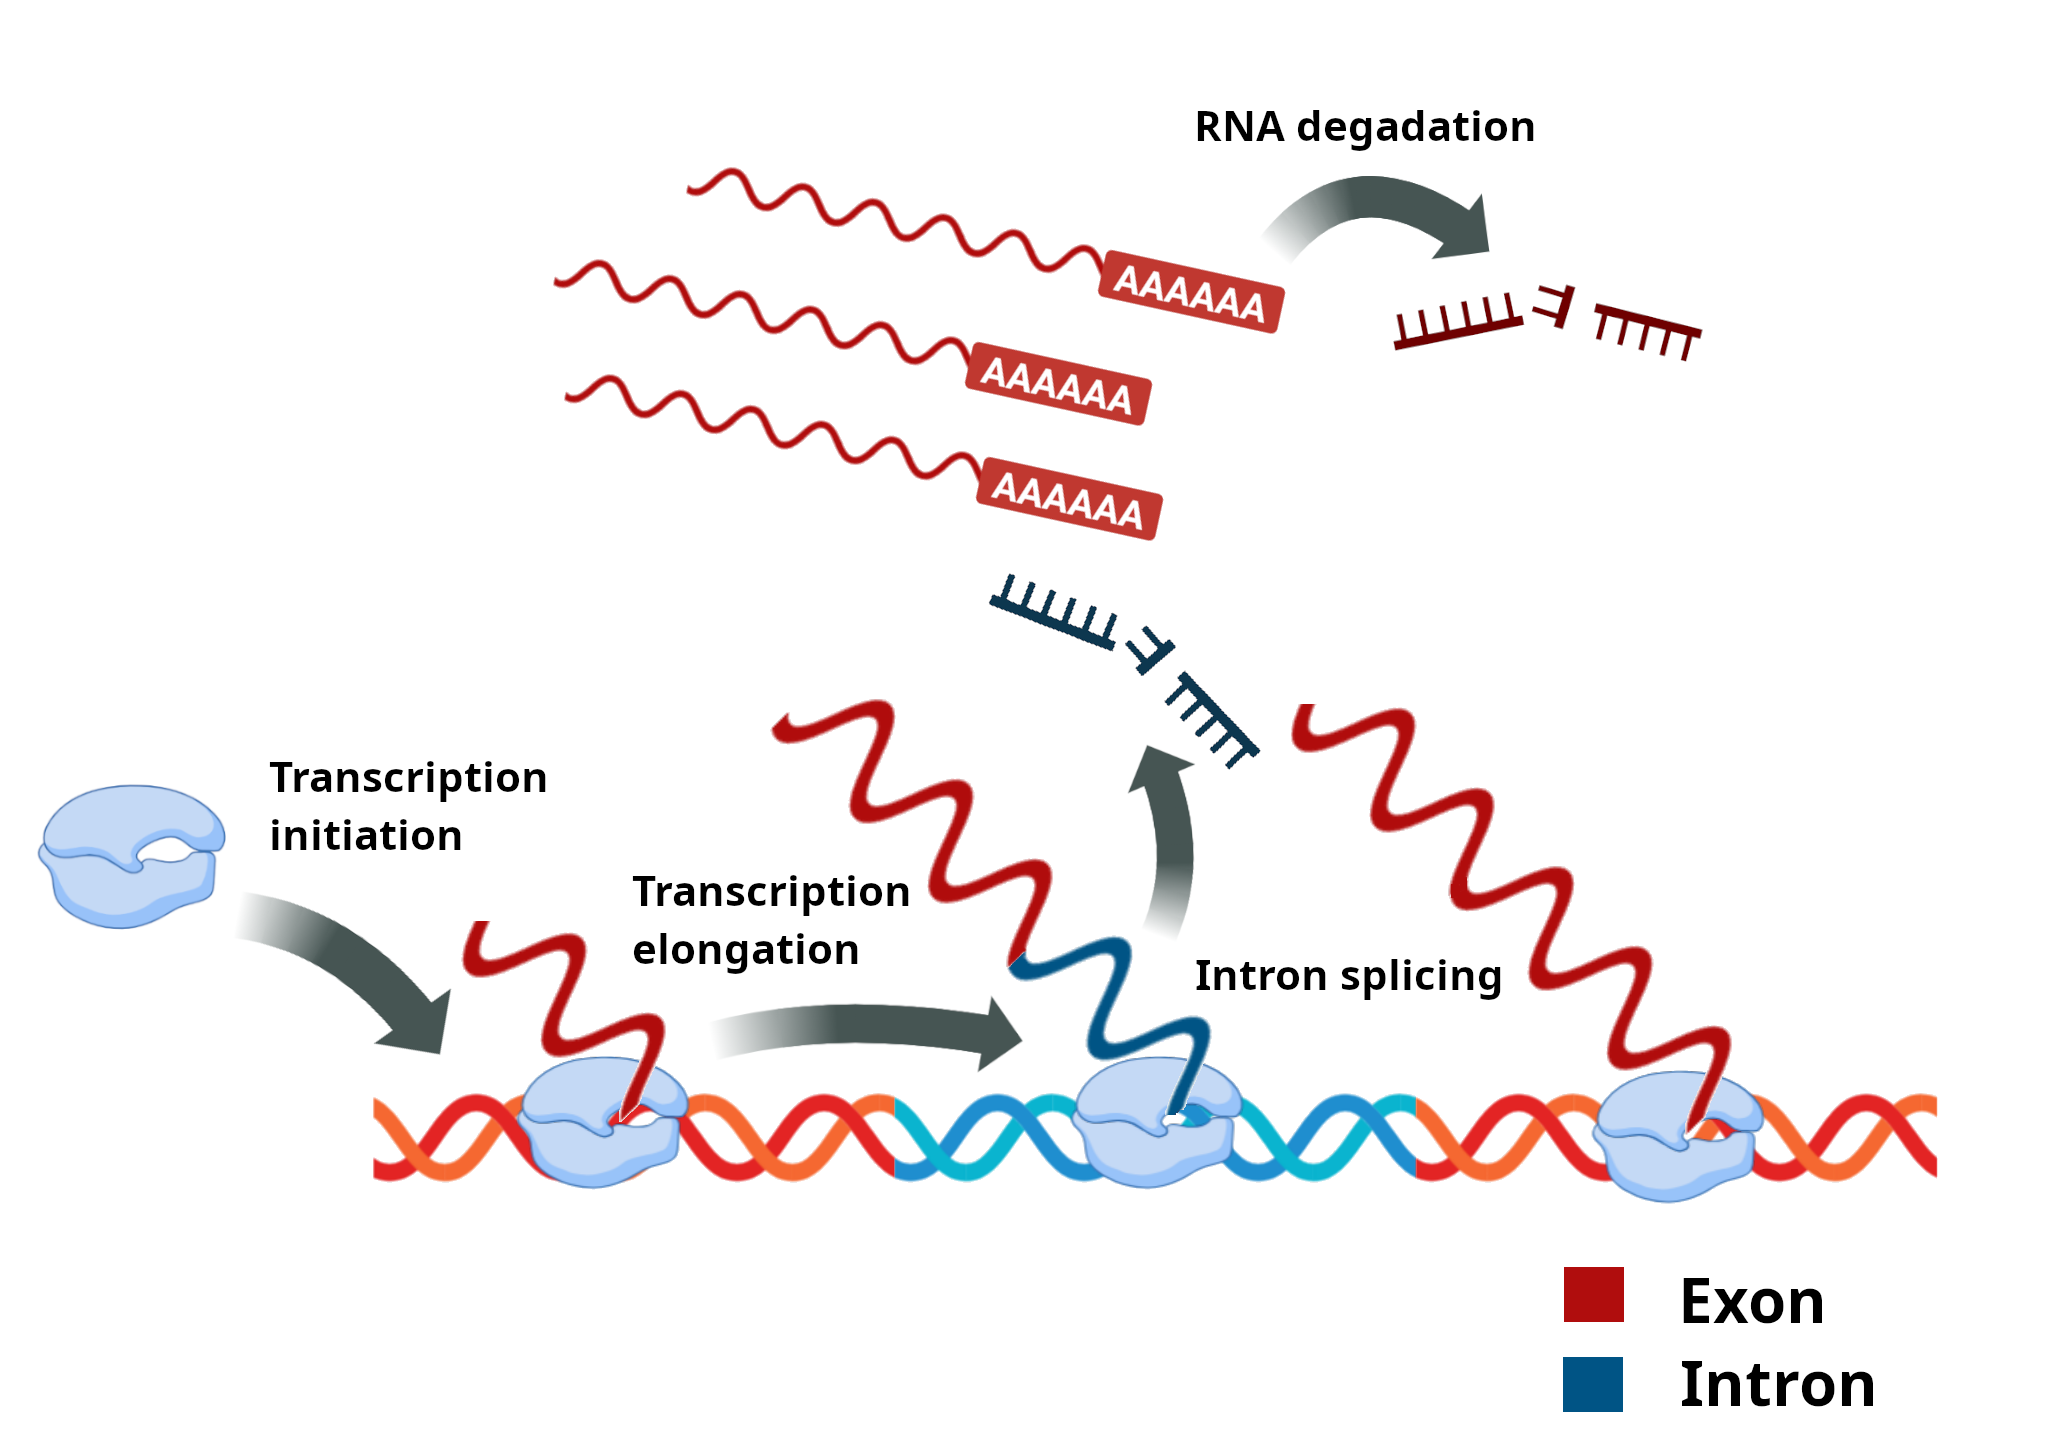
\includegraphics[width=0.9\textwidth]{rna_metabolism.png}
        \caption{Schema of RNA metabolism.}
        \label{fig:rna_metabolism_schema}
    \end{figure}

    Our description focuses only on the processes in the RNA metabolism that can be captured by total RNA-seq data. Other processes, such as nuclear export or translation, are not reflected in total RNA-seq, and we therefore omit them in our model.


    The four processes described in our model - transcription initiation, transcription elongation, intron splicing and RNA degradation - are chemical reactions, and their speeds can be described by the following kinetic parameters:
    \begin{itemize}
        \item The transcription \textbf{initiation rate} $k_{\mathrm{init}}$, measured by the number of polymerases that initiate transcription per second: $\left[ k_{\mathrm{init}} \right]= \mathrm{polymerases}\ \cdot \mathrm{s}^{-1}$.
        \item The transcription \textbf{elongation speed} $k_{\mathrm{elong}}$, measured by the number of base-pairs transcribed per second: $\left[ k_{\mathrm{elong}} \right]= \mathrm{bp}\ \cdot \mathrm{s}^{-1}$.
        \item The intron \textbf{splicing speed} $k_{\mathrm{splice}}$, measured as the inverse of the mean time required for intron splicing and degradation: $\left[ k_{\mathrm{splice}} \right]= \mathrm{s}^{-1}$.

        \item The RNA \textbf{degradation rate} $k_{\mathrm{deg}}$, measured as the inverse of the mean time that a mature transcript will live in a cell: $\left[ k_{\mathrm{deg}} \right]= \mathrm{s}^{-1}$.
    \end{itemize}
    We assume that the kinetic rates may be different for different genes, and that the splicing speed may also vary for different introns in a given gene. Moreover, we assume that the kinetic rates may vary between conditions of the sample (e.g. comparing treated versus control samples), and this variation is what our statistical model (described in the section \nameref{inference_model}) aims to estimate.

    Besides these variations, we assume the kinetic rates to be constant. That is, while our model will describe how abundances of different RNA molecules change in time, the kinetic rates themselves are assumed to stay unchanged. Moreover, we assume that the elongation speed $k_{\mathrm{elong}}$ is constant across the whole gene.

    We also assume the transcription to start only at TSS, and terminate at transcription end site (TES). That is, we assume no cryptic initiation within the gene body, and also no premature termination of the transcription.

    \subsection{State Variables}
    We will describe the model state by the following variables: density of the polymerases transcribing the gene $\rho(x)$, number of mature transcripts $T_{\mathrm{mature}}$, and, for each intron in the gene, the number of fully transcribed but unspliced introns $I_{\mathrm{unspliced}}$. Furthermore, the polymerase density $\rho(x)$ can be used to derive the number of nascent transcripts $T_{\mathrm{nascent}}$ and the number of introns currently being transcribed $I_{\mathrm{nascent}}$. These variables are described in more detail below.

    Each of these variables is a function of time; we omit writing the explicit time argument in this section for the sake of brevity.

    We assume a given gene (in a given biological sample) of a length $L_{\mathrm{gene}}$. The gene length is measured in base-pairs, $\left[ L_{\mathrm{gene}} \right]= \mathrm{bp}$. We consider the gene to be a continuous interval $\left[0, L_{\mathrm{gene}} \right]$.

    The polymerases transcribing the gene are modeled by a continuous density function $\rho(x), x \in \left[0, L_{\mathrm{gene}} \right]$. The density is measured in the number of polymerases per base-pair, $[\rho] = \mathrm{polymerases}\cdot\mathrm{bp}^{-1}$. The density $\rho(x)$ is non-negative, and can be used to obtain the amount of polymerases located in any interval $(a,b)$ as $\int_{a}^{b} \rho(x) dx$.

    Specifically, we will denote the number of nascent transcripts (which is equal to the number of transcribing polymerases) as
    \begin{equation} \label{eq:t_nascent_def}
    T_{\mathrm{nascent}} = \int_{0}^{L_{\mathrm{gene}}} \rho(x) dx
    \end{equation}

    Besides the number of nascent transcripts, we will be also interested in the number of polymerases that currently transcribe given intron. We will consider an intron of length $L_{\mathrm{intron}}$, starting at a location $s$. We denote the amount of nascent introns (i.e., the number of polymerases transcribing the intron) as
    \begin{equation} \label{eq:i_nascent_def}
    I_{\mathrm{nascent}} = \int_{s}^{s+L_{\mathrm{intron}}} \rho(x) dx
    \end{equation}

    We denote the scalar amount of finished transcripts present in the sample as  $T_{\mathrm{mature}}$. We use the term \textit{mature} loosely to mean a transcript whose transcription has finished; while most such transcripts are also fully processed, a fraction may still be undergoing processing (e.g.\ polyadenylation or splicing). We do not model these processing steps explicitly and treat all finished transcripts as a single pool $T_{\mathrm{mature}}$.

    Similarly, for given intron, we denote the amount of finished, but yet unspliced introns as $I_{\mathrm{unspliced}}$. We don't make any assumptions about the transcript in which such unspliced intron is located: the transcript may be nascent, transcribed but not processed yet, or the unspliced intron may be retained in otherwise mature transcript.

    \subsection{Model Dynamics}
    We will now describe the dynamics of our model. For the sake of brevity, we will write the explicit time argument only for the variables that depend also on the location $x$.
    
    To begin with, we define the polymerase flux as 
    \begin{equation} \label{eq:flux_def}
    J(x,t) = k_{\mathrm{elong}} \cdot \rho(x,t)
    \end{equation}
    The flux represents the rate at which polymerases pass the location $x$, and is measured in polymerases per second: $\left[ J \right] = \mathrm{polymerases}\ \cdot \mathrm{s}^{-1}$.
    
    We can now write the dynamics of our model:
    
    \begin{tcolorbox}[
    	colback=white, colframe=black, boxrule=0.4pt, arc=1pt,
    	title=Model dynamics, fonttitle=\bfseries\small,
    	coltitle=black, colbacktitle=white, % subtle: no colored title bar
    	left=6pt, right=6pt, top=4pt, bottom=4pt,
    	]
    	\begin{subequations}
    	\begin{align}
    		J(0,t) &= k_{\mathrm{init}} \label{eq:initiation}\\
    		\frac{\partial \rho(x,t)}{\partial t} &= -\frac{\partial J(x,t)}{\partial x} \label{eq:elongation}\\
    		\frac{d T_{\mathrm{mature}}}{dt} &= J(L_{\mathrm{gene}},t) - k_{\mathrm{deg}} \cdot T_{\mathrm{mature}} \label{eq:mature}\\
    		\frac{d I_{\mathrm{unspliced}}}{dt} &= J(s+L_{\mathrm{intron}},t) - k_{\mathrm{splice}} \cdot I_{\mathrm{unspliced}} \label{eq:splice}
    	\end{align}
    	\end{subequations}
    	
    \end{tcolorbox}
    
    
    We will now discuss the model dynamics in more detail.
   \begin{itemize}
	   \item Equation~\eqref{eq:initiation} describes the \textbf{transcription initiation}. It is a boundary condition for the elongation dynamics~\eqref{eq:elongation} at the start of the gene ($x=0$). It states that polymerases enter the gene at $x=0$ with rate $k_{\mathrm{init}}$.
	   
	   \item Equation~\eqref{eq:elongation} describes the \textbf{transcription elongation}. Polymerases move along the gene at speed $k_{\mathrm{elong}}$, giving rise to the flux $J(x,t)$. Because polymerases are neither created nor destroyed within the gene body, the density at a given location changes only through the imbalance between the flux entering and leaving it — that is, the negative spatial gradient of the flux.	   
	   
	   \item Equation~\eqref{eq:mature} describes \textbf{transcript maturation} and \textbf{degradation}. The production term $J(L_{\mathrm{gene}},t)$ is the flux of polymerases at the gene end, producing newly matured transcripts. The decay term $-k_{\mathrm{deg}} \cdot T_{\mathrm{mature}}$ models
	   their degradation, treating $T_{\mathrm{mature}}$ as a well-mixed pool that decays exponentially.	   
	       
	  \item Equation~\eqref{eq:splice} describes \textbf{intron completion} and \textbf{splicing}. The production term $J(s+L_{\mathrm{intron}},t)$ is the flux of polymerases at the intron end, producing newly completed introns. The decay term $-k_{\mathrm{splice}} \cdot I_{\mathrm{unspliced}}$ models intron splicing and degradation, again as exponential decay.
	    
   \end{itemize}

    \subsection{Steady State Solution} \label{subsec:steady_state}
    We will now derive the steady state solution of our model. Since total RNA-seq provides only a single snapshot in time, our inference model (described in the section \nameref{inference_model}) assumes that the system is at steady state, i.e. the cells are in homeostasis.
    
    To obtain the steady state solution, we set time derivatives of all variables to zero. The full derivation is provided in the \nameref{supplementary_methods}. We obtain the following solution:
    \begin{tcolorbox}[
    	colback=white, colframe=black, boxrule=0.4pt, arc=1pt,
    	title=Steady state solution, fonttitle=\bfseries\small,
    	coltitle=black, colbacktitle=white, % subtle: no colored title bar
    	left=6pt, right=6pt, top=4pt, bottom=4pt,
    	]
    	\begin{subequations}
    	\begin{align}
    		\rho(x) &= \frac{k_{\mathrm{init}}}{k_{\mathrm{elong}}} \label{eq:rho_ss}\\
    		T_{\mathrm{nascent}} &= \frac{L_{\mathrm{gene}} \cdot k_\mathrm{init}}{k_\mathrm{elong}}  \label{eq:t_nas_ss}  \\
    		I_{\mathrm{nascent}} &= \frac{L_{\mathrm{intron}} \cdot  k_\mathrm{init}}{k_\mathrm{elong}}  \label{eq:i_nas_ss}  \\
    		T_{\mathrm{mature}} &= \frac{k_\mathrm{init} }{k_\mathrm{deg}}  \label{eq:t_mat_ss}  \\
    		I_{\mathrm{unspliced}} &= \frac{k_\mathrm{init} }{k_\mathrm{splice}}  \label{eq:i_unspliced_ss}
    	\end{align}
    	\end{subequations}    	
    \end{tcolorbox}
	We will now comment on the steady state solution described above.
	\begin{itemize}
		\item The density $\rho(x)$ is uniform over the whole gene body. Its value scales proportionately with $k_{\mathrm{init}}$ and inversely proportionally with $k_{\mathrm{elong}}$.
		\item The values of $T_{\mathrm{nascent}}$ and $I_{\mathrm{nascent}}$ are obtained by integrating the density $\rho(x)$ over the gene and intron body, respectively. For this reason, they scale proportionally with $L_{\mathrm{gene}}$ and $L_{\mathrm{intron}}$, respectively.
		\item In contrast, $T_{\mathrm{mature}}$ and $I_{\mathrm{unspliced}}$ are pools of fully transcribed molecules, therefore they have no dependence on the gene or intron length. Each of them scales proportionally with the common production rate $k_{\mathrm{init}}$, and inversely proportionately with their corresponding removal rate. The removal rate of mature transcripts is the degradation rate $k_{\mathrm{deg}}$, while the removal rate of unspliced introns is $k_{\mathrm{splice}}$, representing the speed of intron splicing and degradation.
	\end{itemize}
	
    

    \subsection{Structural Non-identifiability}
    
    All steady-state quantities derived above depend on ratios of the kinetic rates, rather than on the individual rates directly. Consequently, observing these steady-state quantities is informative about ratios of the kinetic rates, while the individual rates remain non-identifiable.

    This type of non-identifiability is common in dynamical models of RNA metabolism \citep{furlanDynamicsTranscriptionalPosttranscriptional2021}, rather than being a special property of our model. We illustrate it here using a general ODE system; a more general treatment, which also covers the PDE formulation, is provided in the section \nameref{supplementary_methods}. Consider an autonomous dynamical system with state vector $\boldsymbol{x}$ and dynamics
    \begin{equation} \label{eq:autonomous_ode}
    \frac{d\boldsymbol{x}}{dt} = f(\boldsymbol{x}).
    \end{equation}
    For any $c \in \mathbb{R}_+$, it holds that
    \begin{equation} \label{eq:scaling_invariance}
    f(\boldsymbol{x}) = 0 \Leftrightarrow c \cdot f(\boldsymbol{x}) = 0.
    \end{equation}
    The steady states of the system are defined as the points where $f(\boldsymbol{x}) = 0$; therefore, steady-state observations cannot distinguish the dynamics $f(\boldsymbol{x})$ from $c \cdot f(\boldsymbol{x})$. In a model of metabolism, $c \cdot f(\boldsymbol{x})$ describes a system in which all reactions proceed $c$ times faster than in the system with dynamics $f(\boldsymbol{x})$; both systems share the same steady states, and thus cannot be told apart from steady-state data alone. Because scaling all rates by a common factor leaves the observations unchanged, any identifiable quantity must be unchanged by such scaling, which is exactly the case for ratios of rates.

    Because only ratios of rates are identifiable, comparing biological conditions can reveal changes only in these ratios. As the logarithm of a ratio is a difference of logarithms, the log-fold-change (LFC) of a rate ratio equals the difference of the individual rate LFCs, for example $\mathrm{LFC}(k_{\mathrm{elong}} / k_{\mathrm{deg}}) = \mathrm{LFC}(k_{\mathrm{elong}}) - \mathrm{LFC}(k_{\mathrm{deg}})$. Such differences of LFCs are therefore the quantities that our inference model estimates.

    Finally, we note that the compositional nature of RNA-seq data introduces a second, independent source of non-identifiability. We address it, and describe the resulting estimable quantities in full, in the section \nameref{inference_model}.


    \section{Inference Model} \label{inference_model}
    Here we describe our inference model, working with total RNA-seq data. Throughout this section we retain all modeling assumptions introduced in Section 2, and we assume the system is at steady state.
    
    \subsection{Distinguishing Nascent and Unspliced Introns by Read Coverage}
    
    We will start by discussing the key component of our model: the fact that nascent introns $I_{\mathrm{nascent}}$ and unspliced introns $I_{\mathrm{unspliced}}$ produce different read coverage patterns, which allows us to distinguish them, and consequently identify the ratio $k_\mathrm{elong} / k_\mathrm{splice}$ from the data. This core principle was first observed by \citet{ameurTotalRNASequencing2011}, and subsequently utilized in the work of others \citep{jonkersGenomewideDynamicsPol2014, graySnapShotSeqMethodExtracting2014, kawamuraStatisticalInferenceRate2019, debesAgeingassociatedChangesTranscriptional2023}.
    
    The read coverage can be decomposed into two parts: the location of reads (the 'shape' of coverage), and the amount of reads (the 'scale' of coverage). Here we focus on the shape; the scale enters our model through the read counts, as described below.

    We now consider an intron of length $L_{\mathrm{intron}}$; without loss of generality, we assume that it starts at position $s=0$. We will model each short sequencing read as a point $x \in \left[0, L_{\mathrm{intron}} \right]$. The shape of read coverage can be then described by probability density $p(x)$, specifying the location of reads. Nascent and unspliced introns produce reads with different location distributions; the overall density $p(x)$ is therefore a mixture distribution:
    \begin{equation} \label{eq:mixture}
    p(x) = \pi \cdot p_{\mathrm{nascent}} (x) + (1-\pi) \cdot p_{\mathrm{unspliced}}(x)
    \end{equation}
    where $p_{\mathrm{nascent}}$ is the location distribution of reads from nascent introns, $p_{\mathrm{unspliced}}$ is the location distribution of reads from unspliced introns, and $\pi$ is a mixture coefficient giving the proportion of reads from nascent introns:
    \begin{equation} \label{eq:pi_counts}
    \pi = \frac{I_{\mathrm{nascent}}}{I_{\mathrm{nascent}} + 2 \cdot I_{\mathrm{unspliced}}}
    \end{equation}
    The constant term $2$ accounts for the fact that a nascent intron is, on average, only half transcribed, and therefore produces about half as many reads as a fully transcribed unspliced intron. This follows from the uniform polymerase density \eqref{eq:rho_ss}.

    Plugging in the steady state solution for $I_{\mathrm{nascent}}$ and $I_{\mathrm{unspliced}}$, we obtain:
    \begin{equation} \label{eq:pi_rates}
    \pi = \frac{{L_{\mathrm{intron}} \cdot k_\mathrm{splice}}}{L_{\mathrm{intron}} \cdot k_\mathrm{splice} + 2 \cdot k_\mathrm{elong}}
    \end{equation}
    We also note that $L_{\mathrm{intron}} \cdot k_\mathrm{elong}^{-1}$ is the time needed to transcribe the intron, and $k_\mathrm{splice}^{-1}$ is the time needed to splice it out. Using that, we may also write
    \begin{equation} \label{eq:pi_times}
    \pi = \frac{\text{transcription time}}{\text{transcription time} + 2 \cdot \text{splicing time}}
    \end{equation}

	We will now describe the mixture components $p_{\mathrm{nascent}}(x)$ and $p_{\mathrm{unspliced}}(x)$. We begin with $p_{\mathrm{unspliced}}(x)$: these reads come from fully transcribed introns, and we simply model their location by a uniform distribution
	\begin{equation} \label{eq:p_unspliced}
	p_{\mathrm{unspliced}}(x) = \frac{1}{L_{\mathrm{intron}}}
	\end{equation}
	On the other hand, $p_{\mathrm{nascent}}(x)$ is produced by nascent introns, which have not finished transcribing the intron interval yet. Due to this, reads at location $x$ can be produced only from nascent introns that are already elongated past $x$. This gives us:
	\begin{equation} \label{eq:nascent_density_propto}
	p_{\mathrm{nascent}}(x)  \propto \int_{x}^{L_{\mathrm{intron}}} \rho (z) dz
	\end{equation}
	The steady state solution \eqref{eq:rho_ss} gives a polymerase density $\rho(x)$ that is constant over the gene body. Carrying out the integral in \eqref{eq:nascent_density_propto} and normalizing to a probability density gives us:
	\begin{equation} \label{eq:p_nascent}
	p_{\mathrm{nascent}}(x) = \frac{2 L_{\mathrm{intron}} -2x}{L_{\mathrm{intron}}^2}
	\end{equation}

	The two mixture components thus have distinctly different shapes: a linearly decreasing density for nascent introns, and a uniform density for unspliced introns. The shape of the observed intron coverage is therefore informative about the mixture coefficient $\pi$, and, through \eqref{eq:pi_rates}, about the ratio $k_\mathrm{elong} / k_\mathrm{splice}$.

	We note that the same argument can be also applied to whole transcripts: the fraction of exonic reads originating from nascent transcripts is
	\begin{equation} \label{eq:pi_gene}
		\begin{split}
			\pi_{\mathrm{gene}} &= \frac{T_{\mathrm{nascent}}}{T_{\mathrm{nascent}} + 2 \cdot T_{\mathrm{mature}}}
			= \frac{L_{\mathrm{gene}} \cdot k_{\mathrm{deg}}}{L_{\mathrm{gene}} \cdot k_{\mathrm{deg}} + 2 \cdot k_{\mathrm{elong}}} \\
			&= \frac{\text{gene transcription time}}{\text{gene transcription time} + 2 \cdot \text{mean transcript lifetime}}
		\end{split}
	\end{equation}
	The mature transcripts produce reads with uniform distribution of their location, while nascent transcripts produce reads with coverage decreasing over the gene body, analogously to the case of intron coverage we described above. However, exons may be also spliced out in alternative splicing, which affects the resulting exon coverage and complicates its use for inference.

	For most genes, the transcription time is much shorter than the mean transcript lifetime, and only a few percent of exonic reads therefore originate from nascent transcripts. In our inference model, we neglect the nascent transcript fraction, and assume that all exonic reads are originating from mature transcripts. A further quantification of the effect on our inference model is provided in the section \nameref{supplementary_methods}.
	
	Finally, read coverage is also affected by technical factors, such as read mappability or GC content \citep{derrienFastComputationApplications2012, loveModelingRNAseqFragment2016}. The observed coverage is therefore distorted in a sequence-dependent manner, so that the location distributions derived above are only approximate. As such distortions are determined by the underlying sequence, they affect all samples in the same way; we discuss their impact on our estimates in the section \nameref{supplementary_methods}.
	
	
	
	
	

    \section{Results}
    I will apply the model on some data, e.g. ENCODE datasets of stem cell differentiation, or degron mediated protein KD. Will plot and describe the results here. Should mainly serve for illustration, maybe e.g. mutations known to influence elongation speed (Drosophilla and C. Elegans data, maybe human cell lines if data are available).


    \section{Discussion}
    Discuss stuff here.


    \section*{Code availability}
    An implementation of our method is available at \url{https://github.com/jkoubele/kinetics-from-total-rna}.


    \section*{Acknowledgments}
    This work was funded by the Deutsche Forschungsgemeinschaft (DFG, German Research Foundation)
    under Germany's Excellence Strategy – EXC 2030 – 390661388. \\
    Illustrations were created with BioRender.com.


    \bibliography{references}

    \newpage


    \section*{Supplementary Methods} \label{supplementary_methods}
    Implementation details, more math details, etc.
    
    \subsection*{Dynamic Model}
    
    \begin{itemize}
    	
    	\item Note about constant $k_{elong}$ acroos the gene body:  This is somewhat simplifying assumption, as the elongation speed was reported to vary inside a gene body as well, specifically being slower for the first 10-15 kb and then accelerating downstream \citep{munizRNAPolymeraseII2021}. 
    	
    	\item Note about transcript heterogeneity: ODE (exponential decay term) assumes well-mixed pool of mature transcripts. In some experimental setting, the pool of measured transcripts is not well-mixed: for example, with nascent sequencing via EU-seq, only transcript finished recently are captured. The mature transcripts is such pool may not be degraded exponentially. A model that capture the transcript heterogeneity, e.g. with length of polyA tail serving as transcript 'health-bar', may be more appropriate.
    	
    	\item TODO: Add computation of the steady-state solution
    	
    	\item TODO: non-identifiability statement for PDE (to cover the case of our coupled PDE-ODE model).
    	
    \end{itemize}
    
    

\end{document}
